\chapter{Analysis}
\section{Analysis method}
The goal is to make a data driven decision on how much a \ac{vw} Golf arriving at the dealership should be advertised for,
based on the car's specifications, assuming there is some kind of dependence.
To check whether this dependence exists, the correlations between the specifications and the price are evaluated.
After that, to get a model that predicts the price based on the other attributes, linear regression is used.
Its simplicity when it comes to understanding and calculating the model, as well as interpreting the results, make it well-suited
for this use case.    

\section{Data processing}
\subsection{Preprocessing in \ac{excel}}
First step of preprocessing the data is the reduction to only data points with the value \enquote{\ac{vw} Golf} for the car model attribute. Therefore, the \ac{csv} file containing the raw data is
imported into \ac{excel}, and a filter to the car model column is applied. As some cells are blank for certain attributes, another filter removing the affected rows is set for every column. 

\subsection{Preparations for Orange}
After the previous steps, the data set is still not ready to be processed in Orange. The problem is that certain cells not only contain the actual numeric value but also the 
unit. For example the column of the car's average \ac{mpg} always has the text \enquote{mpg} after the value, causing Orange to not recognize it as 
numeric value. To fix this issue, the \ac{csv} file is opened in a text editor, and its \enquote{Find and replace} functionality is used to replace the unit with blank text.
This is working as the texts,
which have to be removed, only appear in two other places, where they are manually added back. So both the \enquote{mpg} from the average \ac{mpg} column and the \enquote{L}
from the engine size column were removed like this.

\subsection{Processing in Orange}
To understand how each attribute affects the car's price, the correlations are calculated using the Pearson correlation coefficient. 
\begin{figure}[h]
    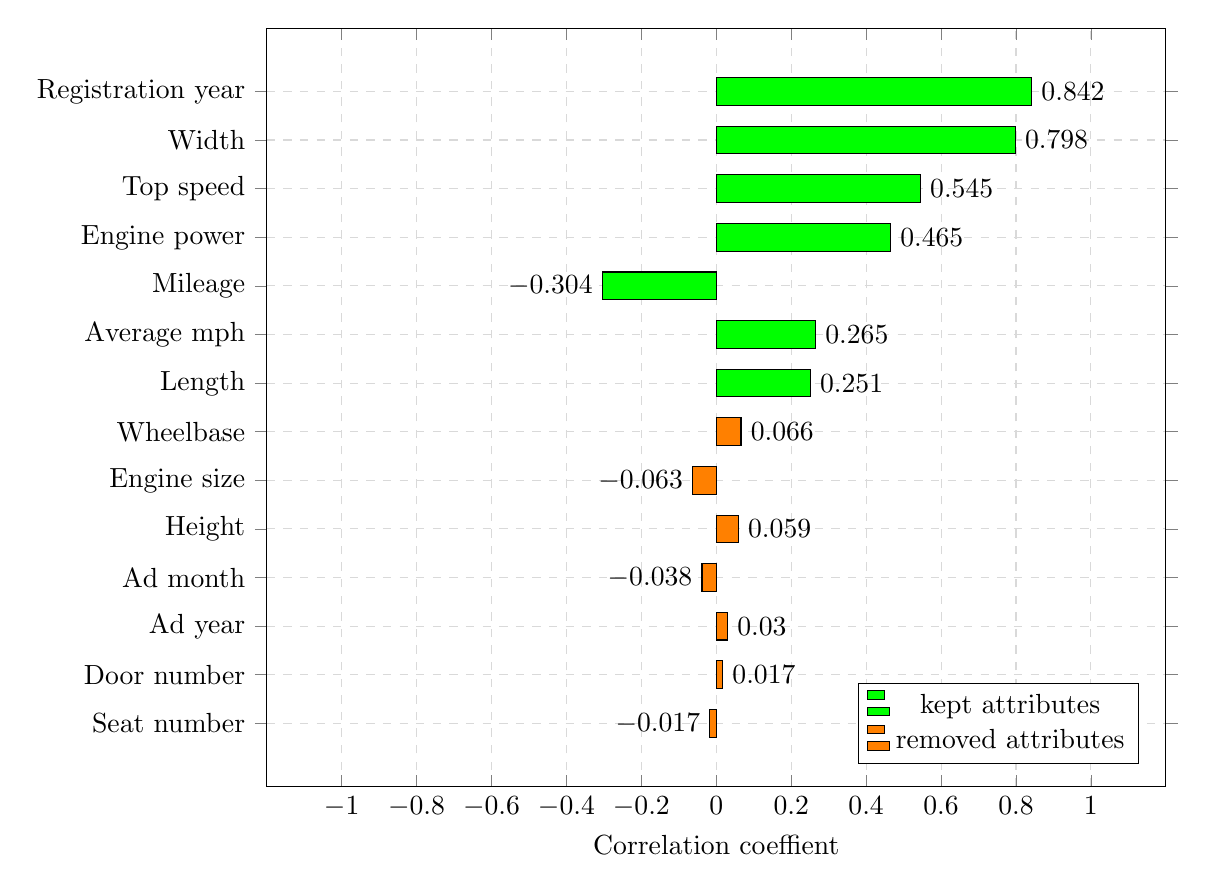
\begin{tikzpicture}
        \begin{axis}[
            xbar,
            xmin=-1.2,
            xmax=1.2,
            xtick={-1,-0.8,-0.6, -0.4, -0.2, 0, 0.2, 0.4, 0.6, 0.8, 1},
            legend pos=south east,
            grid=major, grid style={dashed,gray!30},
            width=13cm,
            xlabel={Correlation coeffient},
            symbolic y coords={Seat number,Door number,Ad year,Ad month,Height,Engine size,Wheelbase,Length,Average mph,Mileage,Engine power,Top speed,Width,Registration year},
            ytick={Seat number,Door number,Ad year,Ad month,Height,Engine size,Wheelbase,Length,Average mph,Mileage,Engine power,Top speed,Width,Registration year},
            nodes near coords,
            nodes near coords align={horizontal},
            every node near coord/.style={/pgf/number format/fixed, /pgf/number format/precision=3},
            /pgf/bar shift={0pt},
            ]
            \addplot [fill=green] coordinates {
                (0.251,Length)
                (0.265,Average mph)
                (-0.304,Mileage)
                (0.465,Engine power)
                (0.545,Top speed)
                (0.798,Width)
                (0.842,Registration year)
                };
            \addplot [fill=orange] coordinates {
                (-0.017,Seat number)
                (0.017,Door number)
                (0.03,Ad year)
                (-0.038,Ad month)
                (0.059,Height)
                (-0.063,Engine size)
                (0.066,Wheelbase)
                };
            \legend{kept attributes, removed attributes}
        \end{axis}
    \end{tikzpicture}
    \caption{Correlation with the price attribute}
    \label{fig:correlationdiagram}
\end{figure}
\par
\autoref{fig:correlationdiagram} shows a horizontal bar chart visualizing the correlation coefficient for each attribute.
As a bar chart lists the different values of the coefficients side by side in an easy-to-read way, it is perfect for the 
given purpose of focusing on comparison between the attributes. 
The horizontal layout allows good readability for the long labels and is more suitable for placing the actual values next to the
bars, as there are no space limitations along the y-axis. 
\par
Having the results of the correlation analysis allows to answer the first research question: \enquote{What factors influence Volkswagen Golf's price the most?}.
\autoref{fig:correlationdiagram} provides the answer, as the attributes are listed from highest to lowest influence on the price. Those highlighted in green
have a significant impact, while the rest do not. Therefore, those highlighted in orange are not taken into account for the further data analysis.

\par
In the next step, not only the attributes with low correlation but also the non-numeric ones are removed. This is the case as they can't be used in the calculation
of the linear regression model without further preprocessing. These additional preprocessing steps are not performed as the resulting linear regression
model is already very good. 
Additionally, the price is set as target value for the linear regression calculation.

\par
As a final step, the data set is split into training and test data, and the linear regression model is calculated based on the
training data. Insights about the training split, as well as quality and specifications of the model, are discussed in the next section of the report. 

\section{Linear regression model}
\subsection{Specifications}
For the calculation of the linear regression model, a training split of 60\% training and 40\% test data is used.
When testing the model, the results are very satisfactory with a \ac{mse} of 3750250.922 and \ac{r2} of 0.912.
Especially, the \ac{r2} being very close to 1 indicates a high linear relationship between the model and the target attribute,
which means that the model predicts the price accurately.

\subsection{Visualization}
The reason for visualizing the linear regression model is that it is always easier to analyze and interpret visual 
results rather than only working with numeric values.
Used for that matter is a scatter plot, shown in \autoref{fig:linearregressiondiagram}. 
\begin{figure}[h]
    \begin{tikzpicture}
        \begin{axis}[
            clip mode=individual,
            legend pos=south east,
            xmin=400,
            xmax=20000,
            ymin=400,
            ymax=20000,
            xlabel={Actual price \lbrack\pounds\rbrack},
            ylabel={Model's calculated price \lbrack\pounds\rbrack},
            xtick={2000, 6000, 10000, 14000, 18000},
            ytick={2000, 6000, 10000, 14000, 18000},
            width=13cm,
            scaled ticks=false,
            tick label style={/pgf/number format/fixed},
            y label style={yshift=1.2em}
            ]
        \addplot [mark=none,color=blue,style=very thick]
          table [y={create col/linear regression={y=model_price}}, col sep=comma] {./other/Linear_regression.csv};
          \addlegendentry{Regression line}  
          \addplot [mark=*,color=red,only marks, fill opacity = 0.35, draw opacity = 0]
          table [x=actual_price, y=model_price, col sep=comma] {./other/Linear_regression.csv};
                 
        \end{axis}
      \end{tikzpicture}
    \caption{Plotted Linear Regression Model}
    \label{fig:linearregressiondiagram}
\end{figure}
\par
Scatter plots are optimal to show the relationship between two variables, in this case, the actual price from the test data 
and the price predicted by the linear regression model. The closer the data points are to the regression line, the 
better the model performs. By knowing this, it is easy to analyze the quality of the model, even without any prior knowledge.
So, when looking at \autoref{fig:linearregressiondiagram}, one can see that the data points portray the regression line 
quite precisely. This reinforces the prior statement that the linear regression model is very good.

